\documentclass[10pt,twocolumn,a4paper]{article}
\usepackage[margin=1.75cm,columnsep=0.62cm]{geometry}
\usepackage{mathptmx}
\usepackage[T1]{fontenc}
\usepackage[utf8]{inputenc}
\usepackage{graphicx,booktabs,microtype,xcolor,caption,url}
\usepackage[hidelinks]{hyperref}

\definecolor{acc}{HTML}{1F4A2E}
\definecolor{rule}{HTML}{9AAE9F}
\captionsetup{font=small,labelfont={bf,color=acc},skip=4pt}
\makeatletter
\renewcommand\section{\@startsection{section}{1}{\z@}%
  {-9pt \@plus -2pt \@minus -1pt}{3pt}%
  {\normalfont\large\bfseries\color{acc}}}
\renewcommand\subsection{\@startsection{subsection}{2}{\z@}%
  {-6pt \@plus -1pt \@minus -1pt}{2pt}%
  {\normalfont\normalsize\bfseries}}
\makeatother
\pagestyle{plain}

\begin{document}

\twocolumn[
\begin{@twocolumnfalse}
\begin{center}
{\LARGE\bfseries\color{acc} Does \texttt{/init} Help?\par}
\vspace{2pt}
{\large A Meta-Study of Repository Context Files for Coding Agents\par}
\vspace{7pt}
{\normalsize\bfseries Marcel Petrick\quad$\cdot$\quad Claude Opus 5\par}
\vspace{2pt}
{\small 19 September 2026\par}
\vspace{7pt}
\begin{minipage}{0.88\textwidth}
\small\noindent\textbf{Abstract.} Agentic coding harnesses ship commands that
generate a repository context file---\texttt{CLAUDE.md}, \texttt{AGENTS.md}---which
is then loaded into every subsequent session. We synthesise the four controlled
ablations of this practice, the surrounding mechanism literature, and primary
sources extracted directly from a shipped Claude Code binary. We find that the
measured effect on task success ranges from $-2\%$ to $+4\%$ and lies entirely
\emph{within} the $\approx$9\% of per-instance outcomes that flip between
byte-identical runs at temperature zero; the field's point estimates therefore do
not distinguish the practice from no practice. The one robust effect is cost,
at $+20$--$23\%$. Decomposing the artefact resolves the apparent disagreement:
\emph{instructions} are followed (a named tool is invoked $1.6\times$ per task
versus $<\!0.01\times$ unmentioned) whereas \emph{repository overviews} are not
helpful, because natural-language summaries of code answer $4/45$ behavioural
questions where the source answers $27/45$---a property of the representation,
not of the author. We argue the pattern follows a general principle:
\textbf{scaffolding decays when it substitutes for a capability the model now has
natively, and persists when it supplies information the model cannot derive or
enforces a constraint it cannot infer.}
\vspace{5pt}
\hrule height 0.5pt
\vspace{9pt}
\end{minipage}
\end{center}
\end{@twocolumnfalse}
]

\section{Introduction}
The practice is near-universal and the evidence is thin. Every major harness
(Claude Code, Codex, Copilot, Cursor, Aider, Gemini CLI, Windsurf, Cline, Amp,
Devin, Junie) ships an instruction-file mechanism; essentially none of their
vendors has published a controlled measurement of whether it works. The entire
causal base is four 2026 preprints, none replicated, none formally rebutted.

We ask three questions. Does a context file improve task success? What does it
cost? And if the answers are ``not measurably'' and ``20\%,'' why does the feature
exist?

\section{Method}
Three rounds of parallel literature search (ten agents) were combined with two
local primary-source efforts: extraction of the literal \texttt{/init} prompt,
an unreleased gated successor, and the loading semantics from the shipped Claude
Code binary v2.1.278; and measurement of 35 instruction files in a working
repository corpus (median $\approx$1{,}590 tokens, p90 $\approx$3{,}300).

Agent output was not trusted. Every load-bearing claim was re-fetched from the
primary source. This caught two passes reporting mutually incompatible figures
from one paper body, one pass reporting $p$-values absent from the paper it cited,
two fabricated statistics in circulation, and one vendor figure absent from its
own source. A full verification log and a self-review of our own first draft
accompany this paper.


\begin{table}[t]
\centering\small
\caption{The complete causal evidence base. All four are 2026 preprints or
workshop papers; none is replicated or formally rebutted. ``Repeats'' denotes
multiple runs of the same condition.}
\label{tab:base}
\begin{tabular}{@{}p{1.45cm}p{1.5cm}p{1.15cm}p{2.5cm}@{}}
\toprule
\textbf{Study} & \textbf{Scale} & \textbf{Repeats} & \textbf{Outcome} \\
\midrule
Gloaguen \cite{gloaguen} & 438 instances, 4 agents & \textbf{No} (1 sample each) & No success gain; $+20$--$23\%$ cost \\
\addlinespace[1pt]
Khatri \cite{khatri} & 288 runs, 17 tasks & \textbf{Yes} ($3\times$) & No effect; but MDE $\approx$30\,pp \\
\addlinespace[1pt]
Lulla \cite{lulla} & 124 PRs, 10 repos & No (paired) & $-28.6\%$ runtime; correctness spot-checked \\
\addlinespace[1pt]
McMillan \cite{mcmillan} & 1{,}650 sessions & \textbf{Yes} ($50\times$) & Affirmative null on file structure \\
\bottomrule
\end{tabular}
\end{table}

\section{Results}

\subsection{The effects are smaller than the noise}
Figure~\ref{fig:forest} plots every measured effect on task success against the
measured run-to-run noise floor. Sam-Bodden~\cite{sambodden}, under a protocol
frozen before data collection, reports that temperature-0 inference ``flips
$\approx$9\% of per-instance outcomes between byte-identical runs,'' and states
this is ``a noise floor under every small effect reported on this benchmark.''
Every published point estimate falls inside it, and the study contributing
several of them sampled each instance once, with no significance testing.

\begin{figure}[t]
\centering
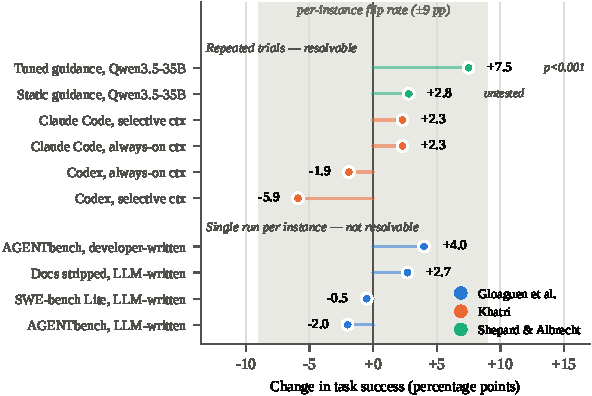
\includegraphics[width=\columnwidth]{fig/fig1_forest.pdf}
\caption{Measured change in task success for every condition in the two
ablations that report success rates, against the $\pm$9\,pp run-to-run noise
floor~\cite{sambodden}. No effect escapes the band.}
\label{fig:forest}
\end{figure}

This is corroborated independently: single runs correlate only $\rho=0.417$ with
true repeated-rollout reliability~\cite{beyondpassk}, and run-level pass rates
overstate retry-free coverage by up to 17.8\,pp~\cite{repeatedrun}. A five-run
replication of one comparison found a single run showing 44\% \emph{slower} where
the five-run median showed 27\% \emph{faster}.

\subsection{Cost is the one robust effect}
Gloaguen et al.~\cite{gloaguen} find inference cost rises 20\% (SWE-bench Lite)
to 23\% (AGENTbench), with 2--4 additional reasoning steps, across every model
tested (Figure~\ref{fig:cost}). Lulla et al.~\cite{lulla} report the opposite
sign---median runtime $-28.6\%$, output tokens $-16.6\%$---but on PRs restricted
to $\leq$100 LOC, with correctness spot-checked on only 50 of 124 cases, leaving
``did less work'' unexcluded.

\begin{figure}[t]
\centering
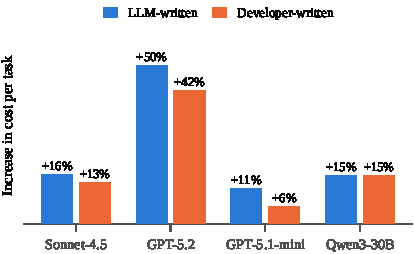
\includegraphics[width=\columnwidth]{fig/fig2_cost.pdf}
\caption{Increase in cost per task on AGENTbench when a context file is present,
by model and provenance. Derived from Table~2 of~\cite{gloaguen}. Unlike the
success-rate effects, this is consistent in sign across all four models.}
\label{fig:cost}
\end{figure}

Cost in tokens is not cost in currency. \texttt{CLAUDE.md} occupies Claude Code's
cached project-context layer; at published rates a 10{,}000-token file costs
\$0.12 across a 50-turn session, and the cached/uncached ratio is exactly
$50/6.15=8.13\times$, independent of file size. \emph{The monetary argument
against a large context file does not survive contact with the arithmetic.}

\subsection{Two artefacts, opposite signs}
The decomposition in~\cite{gloaguen} resolves the field's apparent contradiction:
``instructions in the context files are well followed by coding agents, repository
overviews \ldots are not helpful.'' Instructions move behaviour---a tool named in
the file is invoked $1.6\times$ per instance versus $<\!0.01\times$ unmentioned;
repository-specific tools $2.5\times$ versus $<\!0.05\times$. Overviews do not
measurably reduce steps-to-first-relevant-file, despite appearing in 100\% of
LLM-generated files.

Sam-Bodden~\cite{sambodden} supplies the mechanism and forecloses the obvious
remedy: prose summaries answer $4/45$ behavioural questions about a file where the
source answers $27/45$, and ``the gap belongs to the representation, not the
summarizer---a frontier model's summaries score exactly as poorly as a 3B model's.''
A registered hypothesis that structured skeletons would help \emph{failed}
($N{=}70$, McNemar $p{=}0.75$). Figure~\ref{fig:content} shows that the category
measured not to help is present in roughly two-thirds of real files.

\begin{figure}[t]
\centering
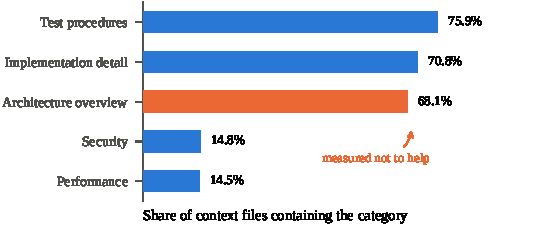
\includegraphics[width=\columnwidth]{fig/fig3_content.pdf}
\caption{Content categories across 2{,}303 context files~\cite{agentreadmes}.
Architecture overviews---the one category with direct evidence of no
benefit~\cite{gloaguen,sambodden}---appear in 68.1\% of files.}
\label{fig:content}
\end{figure}

\subsection{The artefact has no brake}
Across 247{,}694 instruction lifetimes in 1{,}867 repositories, context files grow
\textbf{+226\%} over their lifetime, a net $+4.9$ instructions per commit, and the
older an instruction becomes the \emph{less} likely it is ever
deleted~\cite{chakrabarti}. Appending is cheap; verifying a deletion is safe is
$O(2^{|D|})$. Independently, 23.0\% of such files already contain stale code
references~\cite{treude}. Structural file properties---size, position,
architecture, internal contradiction---show \emph{affirmative} null effects on
adherence (BF$_{10}=0.096$, $0.053$); what degrades compliance is session length,
at $-5.6\%$ odds per generated function~\cite{mcmillan}.

\section{Discussion: why the command exists}
\texttt{/init} shipped in Claude Code's first public build (2025-02-24), so it was
not a patch for an observed deficiency. But its performance rationale has eroded
in step with the harness acquiring cheaper homes for the same content: hooks
(2025-06), subagents (2025-07), Skills and a context-saving Explore subagent
(2025-10), path-scoped rules (2025-12), auto-memory (2026-02). Vendor framing
tracks this exactly, from ``an ideal place'' for documentation with no size limit
(2025-04), to the ``naively dropped into context up front'' half of a hybrid with
just-in-time retrieval (2025-09), to a hard 200-line target with the warning that
``bloated \texttt{CLAUDE.md} files cause Claude to ignore your actual
instructions'' (2026-09). An unreleased successor to \texttt{/init}, recovered
from the binary, opens: ``\texttt{CLAUDE.md} is loaded into every Claude Code
session, so it must be concise---only include what Claude would get wrong without
it.''

The feature also carries rationales that cannot decay: it migrates Cursor, Copilot,
Windsurf, Devin and Cline rule files; it onboards new users to the memory system;
and it produces a human-readable artefact for the team.

\subsection*{A principle}
Derived from an unrelated literature---chain-of-thought~\cite{sprague}, prefill,
verification prompting, minimal agent scaffolds~\cite{agentless}---and found to
predict the present result:

\smallskip
\noindent\fcolorbox{rule}{acc!5}{\begin{minipage}{0.935\columnwidth}\small
\textbf{Scaffolding decays when it substitutes for a capability the model now has
natively; it persists when it supplies information the model structurally cannot
derive, or enforces a constraint it cannot infer.}
\end{minipage}}
\smallskip

\noindent A repository overview substitutes for reading the codebase---and the
agent can now grep. Commands, gotchas and prohibitions supply what no amount of
reading yields. The halves have opposite fates because they are different kinds of
thing.

\section{Verdict}
The practice is sound; the default artefact is not. Run \texttt{/init} as a draft,
then delete the architecture tour---it is the half measured not to help, and it
cannot be fixed by rewriting it. Keep only what the repository cannot state about
itself. Count imperatives rather than lines, since compliance degrades with
constraint count and session length, not file size. Move enforcement to hooks,
procedures to skills, and module detail to path-scoped files; \texttt{@imports}
load eagerly and save nothing. Do not shrink the file to save money---shrink it to
protect compliance. Expect no gain in success rate: agents fail on implementation
skill, and no document repairs that.

\paragraph{Limitations.} Four unreplicated preprints, three underpowered for the
effects they report; no experiment of our own; modelled rather than measured cost
tables; a single binary version; and a search budget exhausted before the final
round. The decisive experiment---ablating instructions against overviews under one
shared success metric---remains unrun, and is cheap.


\section{Open experiments}
The literature's gaps are specific, and several are inexpensive to close.

\begin{enumerate}\setlength{\itemsep}{1pt}\setlength{\topsep}{2pt}
\item \textbf{Halve the file.} Ablate \emph{instructions only} against
\emph{overview only} against \emph{both} and \emph{neither}, under one shared
success metric with repeated runs. Every ingredient exists; the released
AGENTbench harness makes it a week of compute. This is the decisive experiment
and it has not been run.
\item \textbf{Measure all three at once.} No study reports success, cost and
latency together with repeats. Given a $\approx$9\,pp noise
floor~\cite{sambodden}, a design powered for a 5\,pp effect needs roughly
120--200 tasks~\cite{khatri}---large, but not exotic.
\item \textbf{Staleness versus consequence.} Prevalence is
known (23.0\% of files carry stale references~\cite{treude}); the performance
cost of that staleness is not.
\item \textbf{Generalisation.} The evidence is overwhelmingly Python and
TypeScript. Gloaguen et al. themselves caution that Python's weight in training
data ``might\ldots nullify the effect of context files''~\cite{gloaguen}---the
practice may well pay in languages the model knows less well.
\end{enumerate}

\begin{thebibliography}{9}\small
\setlength{\itemsep}{0.5pt}
\bibitem{gloaguen} T.~Gloaguen, N.~M\"undler, M.~M\"uller, V.~Raychev, M.~Vechev.
\emph{Evaluating AGENTS.md: Are Repository-Level Context Files Helpful for Coding
Agents?} MemAgents @ ICLR 2026. arXiv:2602.11988.
\bibitem{sambodden} B.~Sam-Bodden. \emph{What Context Does a Coding Agent Actually
Need to Act?} arXiv:2607.09691, 2026.
\bibitem{khatri} P.~Khatri. \emph{Do Context Files Help Coding Agents? A Two-Agent
Ablation Study on Real Repositories.} arXiv:2607.27250, 2026.
\bibitem{lulla} J.~L.~Lulla et al. \emph{On the Impact of AGENTS.md Files on the
Efficiency of AI Coding Agents.} JAWs @ ICSE 2026. arXiv:2601.20404.
\bibitem{mcmillan} D.~McMillan. \emph{Instruction Adherence in Coding Agent
Configuration Files.} arXiv:2605.10039, 2026.
\bibitem{chakrabarti} K.~Chakrabarti. \emph{Why Does CLAUDE.md Keep Growing?
Catastrophic Remembering in Agentic Coding.} arXiv:2608.11095, 2026.
\bibitem{treude} C.~Treude, S.~Baltes. \emph{Context Rot in AI-Assisted Software
Development.} arXiv:2606.09090, 2026.
\bibitem{arabat} A.~Arabat, M.~Sayagh. \emph{Toward Instructions-as-Code.}
MSR 2026. arXiv:2606.13449.
\bibitem{agentreadmes} P.~Chatlatanagulchai et al. \emph{Agent READMEs: An
Empirical Study of Context Files for Agentic Coding.} arXiv:2511.12884.
\bibitem{beyondpassk} Y.~Jiang et al. \emph{Beyond Pass@k.} arXiv:2608.14711, 2026.
\bibitem{repeatedrun} \emph{Accuracy, Stability, and Repeated-Run Reliability of
LLMs on Deterministic Programming Tasks.} arXiv:2606.00920, 2026.
\bibitem{sprague} Z.~Sprague et al. \emph{To CoT or not to CoT?} ICLR 2025.
arXiv:2409.12183.
\bibitem{agentless} C.~Xia et al. \emph{Agentless: Demystifying LLM-based Software
Engineering Agents.} arXiv:2407.01489.
\end{thebibliography}

\end{document}
